\section{54 - MAT - FA 4.3, AN 4.3 - Design-Center Linz - Matura 2014/15 2. Nebentermin}

\begin{langesbeispiel} \item[0] %PUNKTE DES BEISPIELS
				
	\meinlr{Das Design-Center ist eines der modernen Wahrzeichen der Stadt Linz. Erbaut wurde es von Juli 1991 bis Ende Oktober 1993. Im Jänner 1994 wurde es als Veranstaltungs- und Messezentrum in Betrieb genommen. Die Träger der Konstruktion lassen sich in guter Näherung durch Parabelbögen beschreiben. Die Spannweite der Bögen beträgt ungefähr 72 m, die maximale Höhe der Bögen liegt bei ca. 13 m. Die Grundfläche des Design-Centers ist ein Rechteck mit 200 m Länge und 72 m Breite.}{\begin{center}
		\resizebox{1\linewidth}{!}{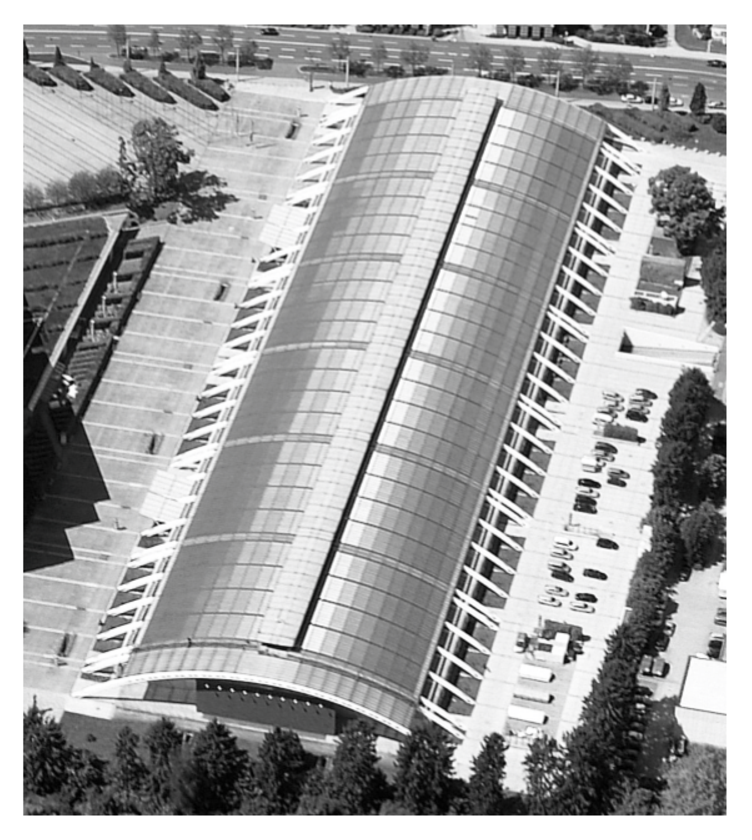
\includegraphics{../_database/Bilder/Bild54-1.eps}}
	\end{center}
	\begin{singlespace}\begin{tiny}Bildquelle: www.linz.at/images/dc\_druck.jpg [09.09.2015]\end{tiny}\end{singlespace}}


\subsection{Aufgabenstellung:}
\begin{enumerate}
	\item Zur Modellierung der parabelförmigen Träger wurde, wie in der folgenden Grafik dargestellt, ein Koordinatensystem durch die Frontansicht des Design-Centers gelegt:
	
	\begin{center}
		\resizebox{0.8\linewidth}{!}{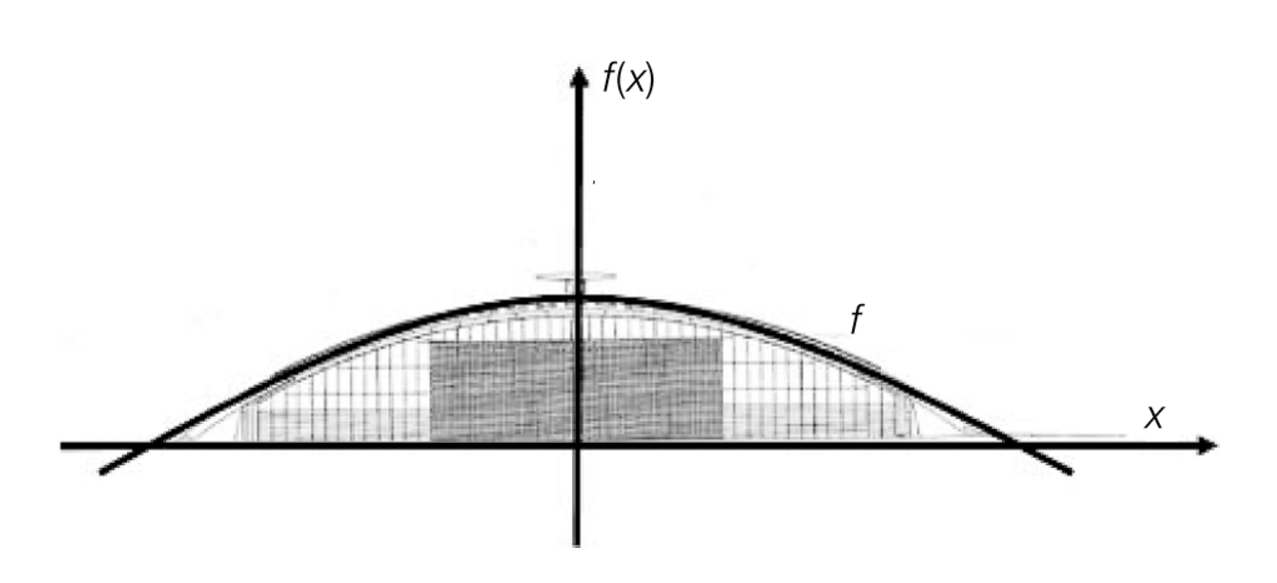
\includegraphics{../_database/Bilder/Bild54-2.eps}}
	\end{center}
	
	\fbox{A} Gib eine Gleichung der Polynomfunktion zweiten Grades $f$ an, welche diese Parabel beschreibt!
	
	Gib an, was durch $200\cdot 2\cdot \int^{36}_0{f(x)}$d$x$ in Bezug auf das Design-Center berechnet wird!\leer
	
\item Die Baukosten für das Design-Center betrugen zur Zeit der Baufertigstellung (1993) umgerechnet ca. \EUR{66} Mio.  

Der Baukostenindex ist ein Maß für die Entwicklung derjenigen Kosten, die Bauunternehmern bei der Ausführung von Bauleistungen durch Veränderungen der Kostengrundlagen (Material und Arbeit) entstehen. Er gibt z.B. an, wie stark die Kosten für Hochbauten pro Jahr steigen. 

Berechne unter der Annahme, dass der Baukostenindex für Österreich 3,5\,\% pro Jahr beträgt, die Höhe der Baukosten für das Design-Center, wenn es erst 10 Jahre später gebaut worden wäre!

Die nachstehende Tabelle gibt Auskunft über die Entwicklung des Baukostenindex der Gesamtbaukosten für den Wohnhaus- und Siedlungsbau im Zeitraum von fünf aufeinanderfolgenden Jahren.

\begin{center}
	\begin{tabular}{|c|c|}\hline
	\cellcolor[gray]{0.9}Jahr&\cellcolor[gray]{0.9}Baukostenindex\\ \hline
	2010&$+3,2\,\%$\\ \hline
	2011&$+2,3\,\%$\\ \hline
	2012&$+2,1\,\%$\\ \hline
	2013&$+1,9\,\%$\\ \hline
	2014&$+1,1\,\%$\\ \hline
	\end{tabular}
\end{center}
\begin{scriptsize} Quelle: http://www.statistik.at/web\_de/statistiken/wirtschaft/preise/baukostenindex/index.html [30.10.2015]\end{scriptsize}

Jemand interessiert sich für den durchschnittlichen Baukostenindex in diesen fünf Jahren. Zur Abschätzung führt er die folgende Rechnung aus:
 $$\frac{3,2+2,3+2,1+1,9+1,1}{5}=2,12$$

Die Vorgehensweise ist für die Berechnung des durchschnittlichen Baukostenindex allerdings nicht ganz korrekt. Gib an, wie diese Berechnung korrekt zu erfolgen hätte!
						\end{enumerate}\leer
				
\antwort{
\begin{enumerate}
	\item \subsection{Lösungserwartung:} 
	
	$f(x)=-\frac{13}{1\,296}\cdot x^2+13$\leer
	
	oder:\leer
	
	$f(x)\approx -0,01\cdot x^2+13$
	
	Durch den angegebenen Term wird das (umbaute) Volumen des Design-Centers berechnet.
		
	\subsection{Lösungsschlüssel:}
	\begin{itemize}
		\item Ein Ausgleichspunkt für das Aufstellen einer korrekten Funktionsgleichung. Äquivalente Funktionsgleichungen sind ebenfalls als richtig zu werten.  
		
		Die Aufgabe ist auch dann als richtig gelöst zu werten, wenn bei korrektem Ansatz das Ergebnis aufgrund eines Rechenfehlers nicht richtig ist.
		\item  Ein Punkt für eine (sinngemäß) korrekte Deutung.
	\end{itemize}
	
	\item \subsection{Lösungserwartung:}
			
		2003 würden die Baukosten für das Design-Center ca. \EUR{93,1} Mio. betragen.\leer
		
		Korrekte Vorgehensweise:
		
		$K\cdot 1,032\cdot 1,023\cdot 1,021\cdot 1,019\cdot 1,011=K\cdot a^5 \Rightarrow$
		
		$a=\sqrt[5]{1,032\cdot 1,023\cdot 1,021\cdot 1,019\cdot 1,011} \Rightarrow a\approx 1,02118$

	\subsection{Lösungsschlüssel:}
	
\begin{itemize}
	\item Ein Punkt für eine korrekte Berechnung.
	
	Toleranzintervall [\EUR{93} Mio.; \EUR{94} Mio.]
	\item Ein Punkt für die Angabe einer korrekten Vorgehensweise. Die numerische Berechnung des Wertes muss dabei nicht erfolgen. 
\end{itemize}

\end{enumerate}}
		\end{langesbeispiel}